\documentclass[12pt, letter]{exam}
\usepackage[utf8]{inputenc}
\usepackage[spanish]{babel}
\usepackage{graphicx}
\usepackage{float}
\usepackage{cite}
\usepackage{natbib}
\usepackage{hyperref}
\usepackage{mdframed}
\mdfdefinestyle{mystyle}{leftmargin=1cm,rightmargin=1cm}
\usepackage{upquote,textcomp}
\newcommand\upquote[1]{\textquotesingle#1\textquotesingle}
\date{}
\title{\begin{LARGE}
{Taller 3 Herramientas Computacionales: \LaTeX \hspace{4pt}- Listas, Figuras y Bibliograf\'ia}
\end{LARGE}}

\begin{document}

\maketitle


La entrega de esta tarea debe contener los siguientes archivos: \verb'verbos.sh', \verb'imagenes.tex' y \verb'referencias.tex'. Nombrar el archivo comprimido con el formato \verb'NombreApellido_HW3.tar.gz'\\

\begin{questions}

\question \framebox{35pts}(Listas) El archivo \verb|verbos-espanol.txt| es una lista de los verbos del idioma espa\~nol en formato de texto plano. Cada l\'inea del archivo es una palabra. Haga un archivo ejecutable que pase el archivo \verb|verbos-espanol.txt| a formato \verb|lista.tex| y que adem\'as compile y genere el archivo \verb|lista.pdf|. Este archivo debe ser un libro de \LaTeX \hspace{1pt} que debe usar el ambiente \verb|\begin{description}| para hacer una lista con los verbos, seguidos de un texto que diga: este es el verbo n\'umero \#. En donde el s\'imbolo \# se reemplaza por la posici\'on del verbo en la lista. Para hacer esto puede hacer uso del comando \verb|sed| que sirve para hacer reemplazos en archivos de texto. Tenga en cuenta lo siguiente:

\begin{itemize}
\item \verb"sed 's/símbolo-a-quitar/símbolo-a-insertar/g'"\\
Toma el archivo de entrada y lo imprime con todas las ocurrencias del símbolo-a-quitar reemplazadas con el símbolo-a-insertar, los caracteres \verb+\+ y \verb+&+ son especiales y deben usarse como se explica más adelante.
\item \verb"sed 's/$/final/g'" \\
Toma el archivo de entrada y pone al final de cada línea el texto ``final''.
\item \verb"sed 's/^/inicio/g'" \\
Toma el archivo de entrada y pone al inicio de cada línea el texto ``inicio''.
\item Si quiere usar el caracter \verb+\+ en \verb+sed+ como parte de un texto tiene que ponerlo de la forma \verb+\\+, por ejemplo, si al final de cada línea quisiera poner \verb+\final+, debería invocar \verb+sed+ de la siguiente forma \verb+sed 's/$/\\final/g'+
\item El caracter \verb+&+ también es un caracter especial en \verb+sed+, siendo así tiene que ponerse de la forma \verb+\&+.
\item La coma \verb+,+  no es un caracter especial, es decir que si quisieran reemplazarse todas las comas con otro caracter se utilizaría el comando \\ \verb+sed 's/,/símbolo a insertar/g'+.
\item Pueden enumerar cada l\'inea con el comando \verb|grep -n '^' nombredelarchivo|.
\item Adem\'as pueden usar el comando \verb|awk| para intercambiar columnas.
\end{itemize}
Asegúrese de entender el funcionamiento de \verb+sed+ y \verb|awk| antes de intentar resolver este ejercicio.
\question \framebox{30pts} (Imágenes) Hacer un archivo \verb"imagenes.tex" que reproduzca lo que se muestra abajo, en la parte donde se hace referencia a la figura (fig.\ 1) no vale escribir literalmente ``fig.\ 1'', tiene que usar el comando \verb+\ref+. 

\DeclareGraphicsExtensions{.pdf,.png,.jpg}

\begin{mdframed}[style=mystyle]
\vspace{0.5cm}
En la fig.\ \ref{fig:Isaac} se muestra un retrato de \textit{Sir Isaac Newton}.

\begin{figure}[H]
\centering
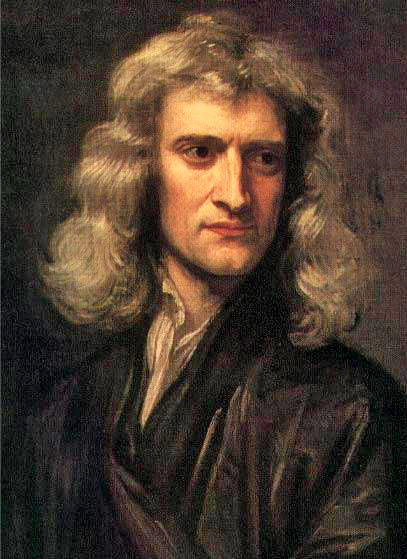
\includegraphics[scale=0.3]{isaac}
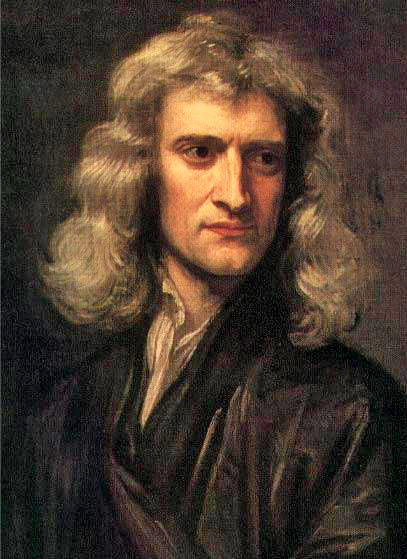
\includegraphics[scale=0.2]{isaac}
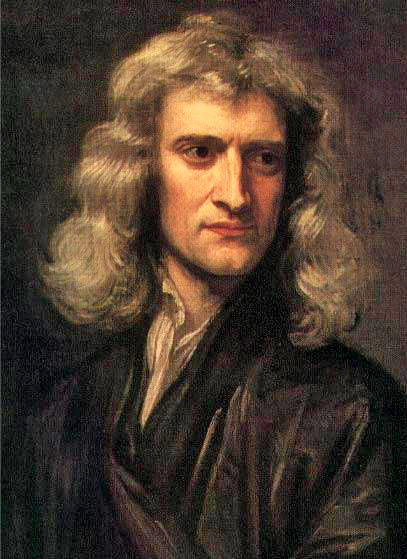
\includegraphics[scale=0.2, angle=100]{isaac}
\caption{Retrato de \textit{Sir Isaac Newton}.}
\label{fig:Isaac}
\end{figure}
\end{mdframed}

\question\framebox{35pts}{(Bibliograf\'ia)} En el archivo \verb"referencias.bib" se encuentra la bibliografía del documento \verb|articulo.pdf|. Cree el archivo \verb+referencias.tex+ donde se reproduzcan los primeros dos p\'arrafos de la introducci\'on del documento \verb|articulo.pdf| con las debidas referencias (excepto la referencia [10]) luego de invocar \verb+pdflatex - bibtex - pdflatex - pdflatex+. En el archivo que se genera, los n\'umeros de las referencias no van a coincidir con los de \verb|articulo.pdf| debido a que no se usan todas las entradas del archivo \verb|referencias.bib|. Aseg\'urese de que en el archivo de \LaTeX \hspace{2pt}utilice los comandos \verb+\bibliography+,\\ \verb+\bibliographystyle+ y \verb+\cite+.

\end{questions}

\end{document}